%!TEX root = Literature_Review_David_Burns.tex

%Todo

% - check your writing style with that writing program
% - get mum to check structure
% - get zoran to check content

%Done

% - put chapters into references
% - read through it for continuity and completeness
% - put in self references where needed


\chapter{Atmosphere}
\label{ch:atmo}

\section{Atmospheric Regions}
\label{sec:atmoreg}

The Earth's atmosphere is split into a number of different layers. The factor governing their division is the sign of the change in temperature with respect to altitude. For example, in \cref{fig:atmolay}, a decrease in temperature ($T$) with an increase in altitude ($z$) in the troposphere occurs up until the tropopause. The difference in temperature gradients between the different levels of the atmosphere prevent mixing from occurring between layers. This occurs as in most circumstances a parcel of air will rise if $\diff{T}{z} < 0$ and fall if $\diff{T}{z} > 0$.

	\begin{figure}[!htb]
	 	\centering
	 	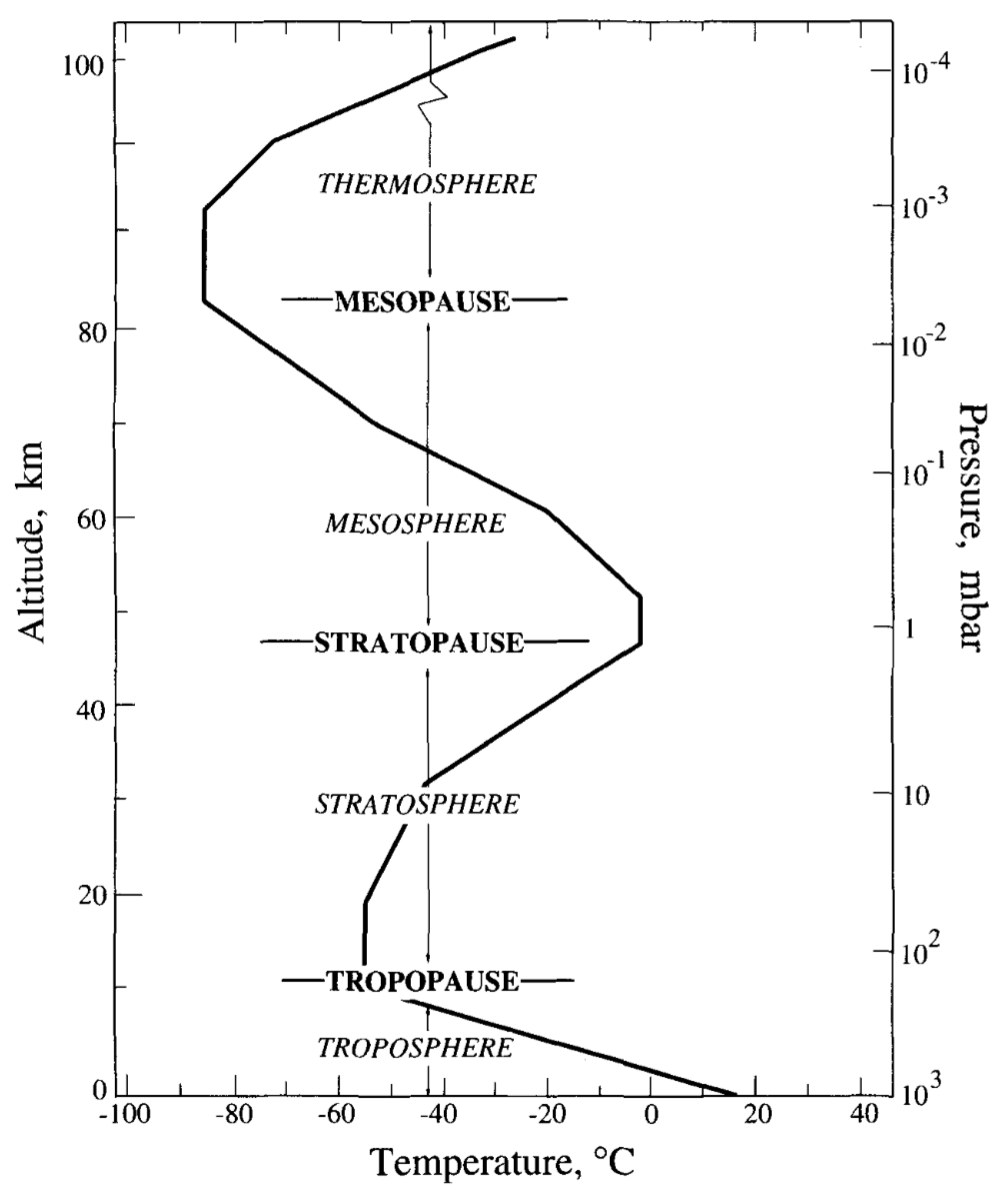
\includegraphics[width=0.8\textwidth,natwidth=1004,natheight=1196]{Fig/Atmosphere_Layers.png}
	 	\caption{The layers of Earth's atmosphere, separated by pauses in temperature change with respect to altitude \citep[p. 7]{seinfeld2012atmospheric}}.
	 	\label{fig:atmolay}
	\end{figure}

\subsection{Troposphere}
\label{subsec:trop}
The troposphere is the lowest level of the atmosphere sitting between $10-15$ \si{\km} above the surface of the Earth. It ends at the tropopause, the first region of constant temperature. The range of altitudes is dependant on time and latitude with the highest region being over the equator, shifting up and down the Earth with its axial tilt \citep[Chapter 1]{seinfeld2012atmospheric}.

The troposphere is an important region as it contains the majority of the atmosphere's mass (approximately \SI{80}{\percent}) and all of its weather. It also contains the highest quantity of water, despite being the smallest region. The layer immediately above the surface of the Earth is called the planetary boundary layer (\gls{pbl}), or marine boundary layer (\gls{mbl}) over the ocean \citep[Chapter 1]{seinfeld2012atmospheric}. The \gls{pbl} varies greatly in height depending on the surface of the Earth it is over, for example, above the Sahara it can be up to \SI{6}{\kilo\meter}, while over tropical oceans it is only \SI{100}{\meter} \citep[Chapter 1]{laing2011introduction}.

There is a short inversion layer in the troposphere that separates the boundary layer and the free troposphere (\gls{ft}) (see \cref{fig:atmolay}). It occurs at only a few hundred metres above tropical oceans \citep{laing2011introduction}. The \gls{ft} is relatively free of aerosols, as the inversion layer prevents mixing with the boundary layer. Thus there is a low aerosol surface area greatly decreasing heterogeneous nucleation. The inversion layer is not always present, and clouds can breach this layer permitting chemicals access into the \gls{ft} from the boundary layer. These conditions promote homogeneous nucleation, which is the formation of new particles \citep[Chapter 8]{seinfeld2012atmospheric}.

\begin{figure}[!htb]
	\centering
	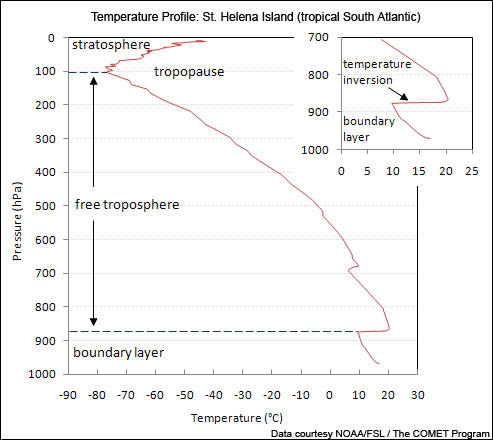
\includegraphics[width=0.8\textwidth,natwidth=493,natheight=440]{Fig/helena_island_skewt.jpg}
	\caption{An example of the separation between \gls{pbl} and \gls{ft} at St. Helena Island. There is an inversion layer present distinguishing the two, however, this obvious separation is not always the case. \citep[Section 1.5.1]{laing2011introduction}}
 	\label{fig:atmolay}
\end{figure}

\section{Relative Humidity and Supersaturation}
\label{subsec:relhum}

The amount of water present in air is usually measured via the relative humidity (\gls{rh}). \gls{rh} is the fraction of the partial pressure of the gas phase water $p_{\text{\tiny H}_2\text{\tiny O}}$ and the saturation vapour pressure for the temperature of the air $p_{\text{\tiny H}_2\text{\tiny O}}^0$, which is the point at which water condenses \citep[Chapter 1]{seinfeld2012atmospheric}. Supersaturation occurs when there is a \gls{rh} greater than \SI{100}{\percent} \citep{rogers1989short}.

\begin{align}
\label{eq:relhum}
	\mathrm{RH} &= 100 \times \frac{p_{\text{\tiny H}_2\text{\tiny O}}}{p_{\text{\tiny H}_2\text{\tiny O}}^0}.
\end{align}

When a parcel of moist air rises in the troposphere the temperature within it decreases which increases the \gls{rh} and a supersaturation can be achieved \citep[Chapter 1]{seinfeld2012atmospheric}. The temperature decreases due to adiabatic expansion. When this occurs water undergoes spontaneous nucleation onto aerosol particles. A seed particle is required for droplet formation to occur; as homogeneous nucleation of water would require a supersaturation far higher than that seen in the atmosphere. \gls{ccn} are the aerosol seeds that droplets form around (see \cref{subsec:ccn}). There is therefore a dependence on the level of supersaturation for an aerosol to act as a \gls{ccn}, which is generally $0.5 - 2$ \si{\percent} \citep[Chapter 6]{rogers1989short}.

% Does the seed particle need to be water soluble?
% i think this is established in the kohler theory paper

\section{Albedo}
\label{sec:albedo}

The albedo of the Earth is given as the ratio between reflected radiation and incident radiation. The amount of light that is not reflected back into space from the surface of the Earth must be absorbed and thus increases the Earth's temperature. Light may be emitted in the infra-red regime as black-body radiation, which either escapes out into space or is absorbed by greenhouse gases in the atmosphere \citep{Lashof:1990wu}. Water acts as a greenhouse gas, but also acts to increase the albedo of the Earth when formed into clouds. A phenomena that alters the amount of light being absorbed by the Earth is said to exhibit radiative forcing \citep{intergovernmentalpanelonclimatechange:2015fa}. Aerosols may cause radiative forcing by either directly reflecting or absorbing light, or by assisting in the formation of clouds \citep[Chapter 4]{seinfeld2012atmospheric}.


%--------------------------------------------------------------------------------------------------------------------------%
%--------------------------------------------------------------------------------------------------------------------------%

	\section{Aerosols}
	\label{sec:aerosols}

	An aerosol is any solid or liquid particle suspended in a gas. In the troposphere there is an abundance of aerosols present, with a vast range of sizes and composition.

	Aerosols are generally subdivided into modes that indicate their production mechanism. When plotting a property of a large number of particles, such as their number or surface area, against the log of the aerosol diameter, peaks appear at different diameters, which are called modes \citep[Chapter 8]{seinfeld2012atmospheric}. The modes are nucleation, Aitken, accumulation, and coarse. The diameters over which these modes are generally found in the atmosphere can be seen in \cref{fig:aermode}.

	\begin{figure}[!htb]
	 	\centering
	 	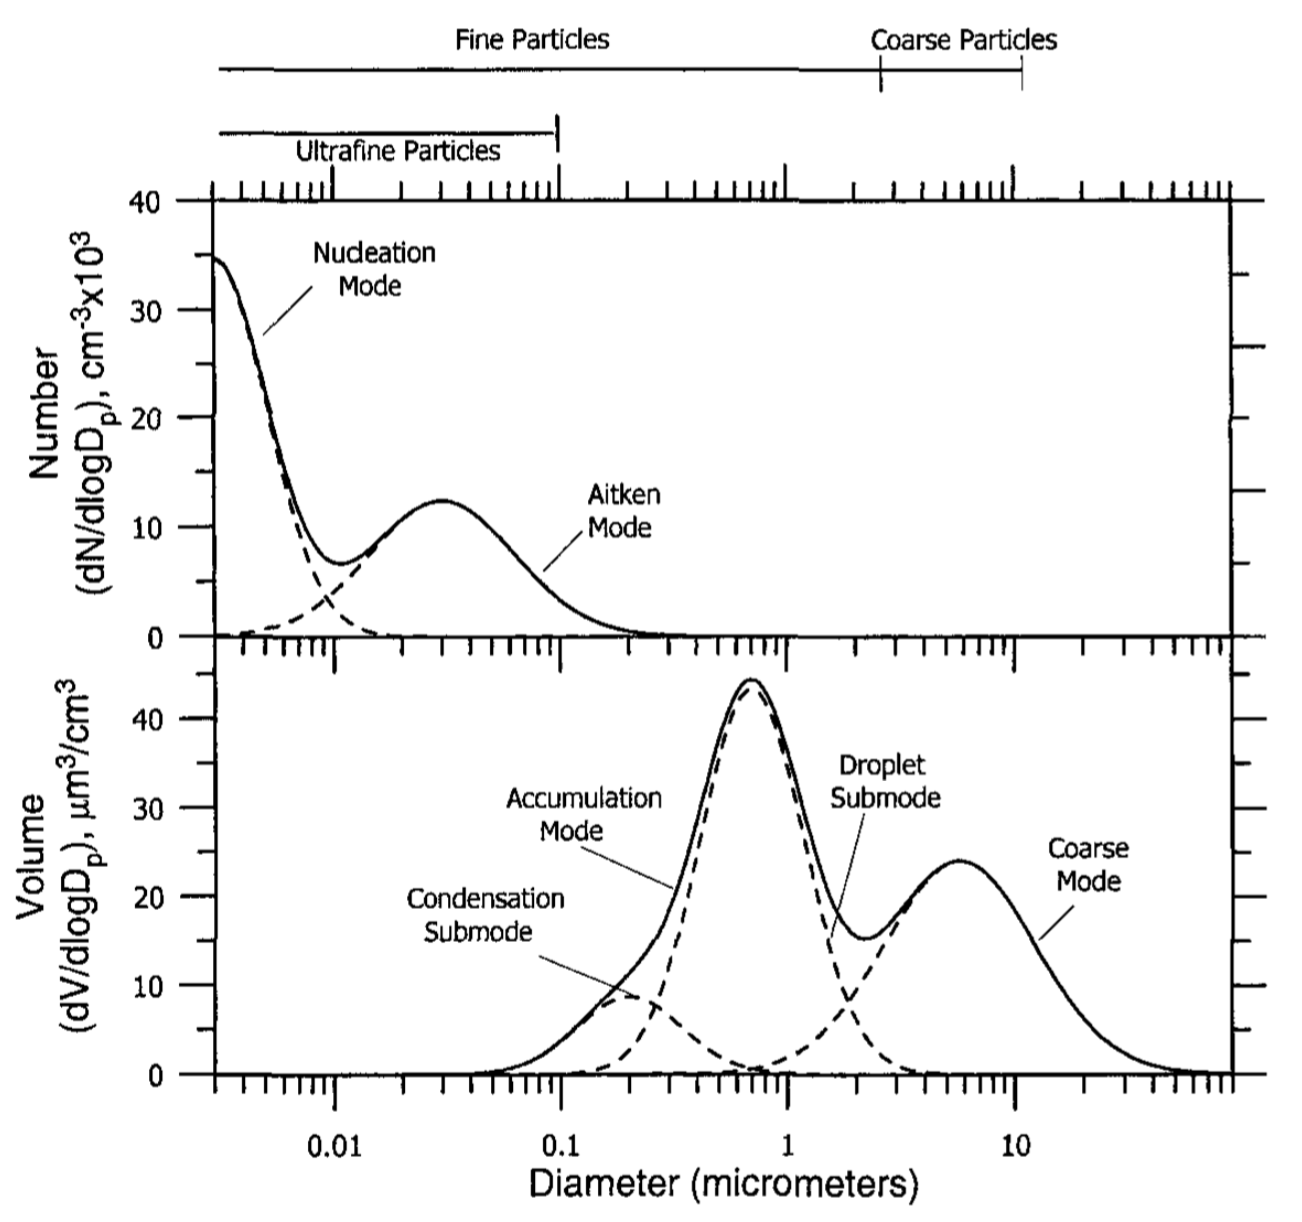
\includegraphics[width=0.8\textwidth,natwidth=1302,natheight=1222]{Fig/aerosolmodes.png}
	 	\caption{A example of the Number and Volume distributions of atmospheric particles indicating the various modes. \citep[Chapter 8]{seinfeld2012atmospheric}}
	 	\label{fig:aermode}
	\end{figure}

	There are many properties of aerosols that can be examined, such as volume, surface area, mass, chemical composition, hygroscopicity, and concentration. For cloud formation the most important characteristics are hygroscopicity, a measure of the particles ability to absorb water, and particle diameter, which governs whether a particle is large enough to act as a \gls{ccn} \citep[Chapter 6]{rogers1989short}. The number, or concentration, of aerosols is important for cloud formation to an extent. If too many \gls{ccn} are present the water vapour concentration may not be high enough to form large droplets \citep[Chapter 22]{seinfeld2012atmospheric}.

	The processes that an aerosol undergoes in the atmosphere dictate some of the modes that appear. The nucleation mode arises from particles homogeneously nucleating from a gas, such as sulphuric acid. The accumulation mode is constructed from particles that have condensed vapour such as water, and/or have grown via coagulation, which occurs when when multiple aerosol particles stick together. The majority of the accumulation mode peak measured in the atmosphere comes from droplet formation in clouds \citep[Chapter 8]{seinfeld2012atmospheric}. This droplet sub-mode can be seen in \cref{fig:aermode}.

	%NSS vs seas salt particles? production and CCN potential?

%--------------------------------------------------------------------------------------------------------------------------%

		\subsection{Particle Formation}

		There are two types of aerosols, primary and secondary. The distinction is based on their method of formation. 

		Primary aerosols are particles that enter the atmosphere directly. In the \gls{mbl} sea salt particles are an example of primary aerosols \citep{quinn:2011iv}.

		Secondary aerosols are aerosols that have formed in the atmosphere via homogeneous nucleation. They begin as gases present in high concentrations, in regions with low concentrations of particles, as heterogeneous nucleation is energetically favourable. Creation of secondary particles are dubbed nucleation events, as the atmospheric conditions required for homogeneous nucleation to proceed are uncommon \citep[Chapter 11]{seinfeld2012atmospheric}. 

		Because nucleation events are rare and localised in time and space they are difficult to simulate, so the percentage of secondary particles on a global scale has a large uncertainty \citep{intergovernmentalpanelonclimatechange:2015fa}. \citet{merikanto:2009iu} modelled global \gls{ccn} production using the \gls{glomap} model and showed that between \SI{31}{\percent} and \SI{49}{\percent} of \gls{ccn} are secondary particles. Approximately \SI{35}{\percent} of these secondary particles were formed in the free and upper troposphere and entrained down into the \gls{mbl} \citep{merikanto:2009iu}.

		% What theory governs nucleation? 
		% Classical vs experimental?

		% \subsection{Marine Aerosols}

		% In the remote ocean aerosols come from a number of different sources. Sea salt is aerosolised through bubble bursting along with primary organic aerosols \citep{cainey:2007jj}. Secondary aerosols are formed from chemicals in the atmosphere, predominantly in the free troposphere \citep{woodhouse:2010ed}. There are also other external sources such as anthropogenic aerosols from shipping or land sources depending on remoteness.

		% The prevalance and effect of aerosols in the remote marine region is the subject of much research and contention \cite{cainey:2007jj}, \citep{quinn:2011iv} \citep{woodhouse:2010ed} \cite{odowd:2007gj}.

%--------------------------------------------------------------------------------------------------------------------------%

		\subsection{CCN}
		\label{subsec:ccn}

		\gls{ccn} are aerosols that are able to act as sites for the heterogeneous nucleation of water. The water droplets continue to grow by precipitating gas phase \gls{h2o} and eventually become massive enough that they fall out of the sky as rain. The formation of clouds requires \gls{ccn}, as the atmospheric conditions for homogeneous nucleation of water are never reached. So \gls{ccn} act as sites for the heterogeneous nucleation of water, forming cloud droplets \citep[Chapter 17]{seinfeld2012atmospheric}. 

		\gls{ccn} are defined for particular supersaturations. This is because whether an aerosol (with a given composition) can act as a \gls{ccn}, is dependant on the supersaturation of the air it is in. The chemical composition of the particle, or it's hygroscopicity, also affect its ability to act as a \gls{ccn}. As this information is not always known, empirical equations are often used to describe the concentration of \gls{ccn}. Take the following equation,
		\begin{align}
			\label{eq:ccnemp}
			\mathrm{CCN}(s) &= cs^k.
		\end{align}
		Here the concentration of \gls{ccn} is given as a power function of supersaturation $s$, where $c$ and $k$ are empirical parameters that conceal the size and composition dependence of \gls{ccn}. The empirical parameters are sampled locationally with $c$ varying between $25 - 3500$ \si{\per\cubic\centi\metre} and $k$ varying between $0.3 - 1.4$ \citep[Chapter 17]{seinfeld2012atmospheric}. If size distributions, composition and supersaturation are known, then K\"{o}hler theory (see \cref{subsec:kohler}) predicts which aerosols may act as \gls{ccn} \citep{rissman:2006ha}.

		\subsubsection{Sources and Sinks for \gls{ccn}}

		There are a number of \gls{ccn} sources. Sea salt is an excellent \gls{ccn} due to its high hygroscopicity \citep{randles:2004ke}. It is also abundant in atmospheric regions above the ocean and coastline. It is aerosolised by bubble bursting and wind shear at the surface of the ocean. 

		Chemicals produced by living organisms can pass through a series of chemical reactions and a subsequent nucleation event to produce \gls{ccn}. An example of this is \gls{dms} produced by phytoplankton, which is further explored in \cref{ch:dms}. An alternative to \gls{dms} derived organic aerosols is dissolved organic matter from dying biota collected at the surface that is aerosolised through bubble bursting \citep{bigg:2007er}. 
		
		There are also a number of anthropogenic sources of \gls{ccn}, however, in the Great Barrier Reef region, only sources from shipping exhaust are likely to be of consequence \citep{fischer2012atmospheric}.

		Aerosols are readily removed from the atmosphere by rainfall and this is even more apparent for \gls{ccn} as they provide the site of droplet formation. Rain also collects aerosols as the droplets fall \citep{rogers1989short}. Deposition onto other aerosol particles is another way in which \gls{ccn} may be removed while it is also possible for aerosols to deposit directly onto the surface of the Earth \citep[Chapter 9]{seinfeld2012atmospheric}.

		\subsection{K\"{o}hler Theory}
		\label{subsec:kohler}
			K\"{o}hler theory was first described in a paper written by the theory's namesake Hilding K\"{o}hler \citep{kohler:1936dq}. It provides a model for the growth of existing particles by heterogeneous nucleation. There are two forces influencing this behaviour, the attraction of a molecule's neighbours (the Kelvin effect), and the concentration of the solution (the solute effect) \citep{rogers1989short}.

			For a particle of diameter $D_p$, the log of the ratio between the water vapour pressure of a droplet and a flat surface is given as a function of the molecular mass of water $M_w$, the surface tension $\sigma_w$, the gas constant $R$, the temperature $T$, the water density $\rho_w$, and the number of moles of the solute $n_s$.
			\begin{align}
				\ln \left(\frac{p_w(D_p)}{p^\circ}\right) &= \frac{4 M_w \sigma_w}{R T \rho_w D_p} - \frac{6 n_s M_w}{\pi \rho_w D_p^3}.
				\label{eq:kohler}
			\end{align}

			Substituting in the known constants produces $\frac{4 M_w \sigma_w}{R T \rho_w} \approx \frac{0.66}{T}$ and $\frac{6 n_s M_w}{\pi \rho_w} \approx \frac{\num{3.44e13} v m_s}{M_s}$ with units \si{\micro\meter} \citep[p. 770]{seinfeld2012atmospheric}. The moles of solute $n_s$ is given by the ratio between the number of ions per molecule $v$, the solute particle mass $m_s$ and the solute molar mass $M_s$. Substituting into \cref{eq:kohler} gives,
			\begin{align}
				\frac{p_w(D_p)}{p^\circ} &= e^{\frac{0.66}{T D_p}} e^{-\frac{\num{3.44e13} v m_s}{M_s D_p^3}}.
				\label{eq:kohlerapp}
			\end{align}
			Here the first exponential term represents the Kelvin effect and the second represents the solute effect.

			Plotting \cref{eq:kohlerapp} produces K\"{o}hler curves that show, for an initial dry particle size, the required supersaturation for particle growth to occur even as the particle itself grows and changes concentration. An example of K\"{o}hler curves for different seed diameters of ammonium sulphate \gls{amsu} can be seen in \cref{fig:kohleras}. Here, \cref{eq:kohlerapp} has been plotted with $v = 3$, $M_s = \SI{132.14}{\gram\per\mole}$.

			\begin{figure}[!htb]
			    \centering
			    \includegraphics[width=0.8\textwidth]{Fig/as_Kcurve.eps}
			    \caption{The K\"{o}hler curves for ammonium sulphate \gls{amsu} for three dry diameters $0.05$, $0.1$, $0.5$ \si{\micro\meter} using approximations from \citet[p. 770]{seinfeld2012atmospheric} }
			    \label{fig:kohleras}
			\end{figure}

			% 'maybe we shouldnt bother with the figure below, we would need a whole bunch more explanation for where the equations come from for it :('

			% \begin{figure}[htpb]
			%     \centering
			%     \includegraphics[scale=0.43]{Fig/as_GvH.eps}
			%     \caption{Growth factor as a function of Relative Humidity for Ammonium Sulphate $(\mathrm{NH}_4)_2\mathrm{SO}_4$ for dry diameter $0.03$ \SI{}{\micro\meter} using approximations from \citet{tang1994water}. Data for comparison comes from \citet{Hameri:2000tc}.}
			%     %\label{fig:}
			% \end{figure}

			There are a number of variations to the general form of the K\"{o}hler curve equation that deal with alternate conditions, such as insoluble seed particles, and mixes of soluble and insoluble seeds \citep[Chapter 17]{seinfeld2012atmospheric}.
